\documentclass[aspectratio=169,11pt]{beamer}

% ---------- Theme ----------
\usetheme[numbering=fraction]{metropolis}
\setbeamertemplate{caption}{\raggedright\insertcaption\par}

% ---------- Packages ----------
\usepackage[T1]{fontenc}
\usepackage{lmodern}
\usepackage{amsmath,amssymb}
\usepackage{booktabs}
\usepackage{graphicx}
\usepackage{multicol}
\usepackage{hyperref}
\usepackage{caption}

% ---------- Metadata ----------
\title{Model Compression and Efficiency Optimisation\\for Edge Deployment}
\subtitle{Diploma Seminar 2 --- Presentation 1\\Research Objective, Methodology, and Validation Plan}
\author{Hubert Jaczynski}
\institute{
  Warsaw University of Technology\\
  \vspace{1mm}
  \footnotesize Supervisor: PhD. Maria Ganzha
}
\date{Warsaw, 2026}

% ---------- Helpers ----------
\newcommand{\noteTime}[1]{\note{\textbf{Timing:} #1}}

% ---------- Single-file bibliography ----------
\begin{filecontents*}{refs.bib}
@article{lecun2015deep,
  title={Deep learning},
  author={LeCun, Yann and Bengio, Yoshua and Hinton, Geoffrey},
  journal={Nature},
  volume={521},
  number={7553},
  pages={436--444},
  year={2015}
}
@article{cheng2017compression,
  title={A survey of model compression and acceleration for deep neural networks},
  author={Cheng, Yu and Wang, Duo and Zhou, Pan and Zhang, Tao},
  journal={arXiv:1710.09282},
  year={2017}
}
@article{gholami2021quant,
  title={A survey of quantization methods for efficient neural network inference},
  author={Gholami, Amir and Kim, Sehoon and Dong, Zhen and others},
  journal={arXiv:2103.13630},
  year={2021}
}
@inproceedings{han2016deepcompression,
  title={Deep compression: Compressing deep neural networks with pruning, trained quantization and huffman coding},
  author={Han, Song and Mao, Huizi and Dally, William J.},
  booktitle={ICLR},
  year={2016}
}
@article{hinton2015distill,
  title={Distilling the knowledge in a neural network},
  author={Hinton, Geoffrey and Vinyals, Oriol and Dean, Jeff},
  journal={arXiv:1503.02531},
  year={2015}
}
@inproceedings{cai2019proxylessnas,
  title={ProxylessNAS: Direct neural architecture search on target task and hardware},
  author={Cai, Han and Zhu, Ligeng and Han, Song},
  booktitle={ICLR},
  year={2019}
}
@article{sze2017efficient,
  title={Efficient processing of deep neural networks: A tutorial and survey},
  author={Sze, Vivienne and Chen, Yu-Hsin and Yang, Tien-Ju and Emer, Joel},
  journal={arXiv:1703.09039},
  year={2017}
}
@incollection{Abid2022EdgeDevices,
  author    = {Abid, Areeba and Sinha, Priyanshu and Harpale, Aishwarya and Gichoya, Judy and Purkayastha, Saptarshi},
  title     = {Optimizing Medical Image Classification Models for Edge Devices},
  booktitle = {Distributed Computing and Artificial Intelligence, Volume 1: 18th International Conference},
  editor    = {Matsui, Kenji and Omatu, Sigeru and Yigitcanlar, Tan and Gonzalez, Sara Rodriguez},
  series    = {Lecture Notes in Networks and Systems},
  volume    = {327},
  pages     = {77--87},
  publisher = {Springer},
  address   = {Cham},
  year      = {2022},
  doi       = {10.1007/978-3-030-86261-9_8}
}
@inproceedings{Redmon2016YOLO,
  title={You Only Look Once: Unified, Real-Time Object Detection},
  author={Redmon, Joseph and Divvala, Santosh and Girshick, Ross and Farhadi, Ali},
  booktitle={Proceedings of the IEEE Conference on Computer Vision and Pattern Recognition (CVPR)},
  year={2016}
}
@article{Tan2020EfficientDet,
  title={EfficientDet: Scalable and Efficient Object Detection},
  author={Tan, Mingxing and Pang, Ruoming and Le, Quoc V.},
  journal={arXiv preprint arXiv:1911.09070},
  year={2020}
}
@article{Howard2017MobileNets,
  title={MobileNets: Efficient Convolutional Neural Networks for Mobile Vision Applications},
  author={Howard, Andrew G. and Zhu, Menglong and Chen, Bo and Kalenichenko, Dmitry and Wang, Weijun and Weyand, Tobias and Andreetto, Marco and Adam, Hartwig},
  journal={arXiv preprint arXiv:1704.04861},
  year={2017}
}
@inproceedings{Liu2016SSD,
  title={SSD: Single Shot MultiBox Detector},
  author={Liu, Wei and Anguelov, Dragomir and Erhan, Dumitru and Szegedy, Christian and Reed, Scott and Fu, Cheng-Yang and Berg, Alexander C.},
  booktitle={European Conference on Computer Vision (ECCV)},
  year={2016}
}
@inproceedings{Carion2020DETR,
  title={End-to-End Object Detection with Transformers},
  author={Carion, Nicolas and Massa, Francisco and Synnaeve, Gabriel and Usunier, Nicolas and Kirillov, Alexander and Zagoruyko, Sergey},
  booktitle={European Conference on Computer Vision (ECCV)},
  year={2020}
}
@inproceedings{Lin2014COCO,
  title={Microsoft COCO: Common Objects in Context},
  author={Lin, Tsung-Yi and Maire, Michael and Belongie, Serge and Hays, James and Perona, Pietro and Ramanan, Deva and Doll{\'a}r, Piotr and Zitnick, C. Lawrence},
  booktitle={European Conference on Computer Vision (ECCV)},
  year={2014}
}
\end{filecontents*}

\usepackage[backend=bibtex,style=numeric,sorting=none]{biblatex}
\addbibresource{refs.bib}

% ---------- Document ----------
\begin{document}

\maketitle
\noteTime{0:00--0:30. State the problem, objective, and what changed since Seminar 1.}

\begin{frame}{Agenda}
\begin{enumerate}
  \item Research problem and objective
  \item Why the problem matters in edge deployment
  \item Methodology and research design
  \item Planned models and optimisation methods
  \item Planned solution architecture
  \item Implementation plan
  \item Validation and evaluation strategy
  \item Current status and discussion points
\end{enumerate}
\noteTime{0:30--1:10. This deck is about the plan, but with enough technical detail to justify the choices.}
\end{frame}

\begin{frame}{Research problem}
\begin{itemize}
  \item Modern object detection models are accurate, but often too heavy for \textbf{resource-constrained edge devices}.
  \item In practice, deployment is limited by:
  \begin{itemize}
    \item inference latency / FPS,
    \item memory footprint and model size,
    \item hardware- and runtime-dependent efficiency.
  \end{itemize}
  \item The key challenge is to improve efficiency \textbf{without making detection quality unusable}.
\end{itemize}

\vspace{2mm}
\noteTime{1:00--1:50. Short motivation only; the focus is the research plan.}
\end{frame}

\begin{frame}{Why edge deployment is difficult}
\begin{itemize}
  \item Edge devices do not only have lower compute than servers. They also have:
  \begin{itemize}
    \item tighter RAM limits,
    \item stricter real-time constraints,
    \item device-specific runtime limitations,
    \item in some cases power or battery constraints.
  \end{itemize}
  \item Therefore, a model with good benchmark accuracy may still fail in practice.
  \item The deployment target is a \textbf{full system problem}: model architecture, precision, runtime, and hardware all matter together.
\end{itemize}
\end{frame}

\begin{frame}{Edge Devices}
\begin{figure}
    \centering
    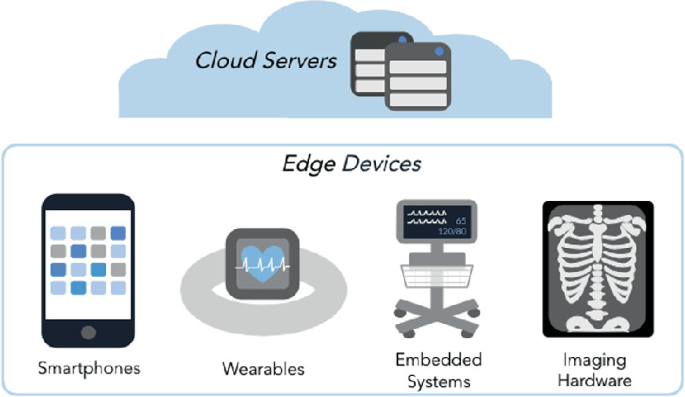
\includegraphics[width=0.7\linewidth]{../img/edge_devices.png}
    \caption{Examples of edge-device variants \cite{Abid2022EdgeDevices}.}
\end{figure}
\noteTime{1:50--3:00. Reuse the visual from Seminar 1, but now connect it directly to the research design.}
\end{frame}

\begin{frame}{Precise research objective}
\begin{block}{Main objective}
Identify which model compression and efficiency optimisation techniques, or combinations of techniques,
provide the best \textbf{accuracy--latency--size trade-off} for real-time object detection on constrained hardware.
\end{block}

\begin{itemize}
  \item \textbf{What I am solving:} detectors are often not directly deployable on edge hardware.
  \item \textbf{What I want to achieve:} a reproducible comparison of selected optimisation strategies under realistic deployment conditions.
  \item \textbf{What success means:}
  \begin{itemize}
    \item a clear evaluation protocol,
    \item a compressed or efficient detector that meets a practical latency budget,
    \item limited accuracy degradation relative to the baseline,
    \item conclusions about which methods work best for the chosen hardware/runtime.
  \end{itemize}
\end{itemize}
\noteTime{1:50--3:00. This is the central slide for both methodology and later evaluation.}
\end{frame}


\begin{frame}{What success means in this thesis}
\begin{itemize}
  \item Success is not only obtaining a smaller model.
  \item The thesis should produce:
  \begin{itemize}
    \item a well-justified baseline model,
    \item a reproducible optimisation and benchmarking procedure,
    \item at least one optimisation path that improves deployment usefulness,
    \item conclusions about the trade-offs between compression methods.
  \end{itemize}
  \item In practical terms, a successful result should show that:
  \begin{itemize}
    \item latency or FPS improves meaningfully,
    \item model size decreases,
    \item accuracy degradation remains acceptable,
    \item conclusions are based on measurements from the target runtime.
  \end{itemize}
\end{itemize}
\noteTime{5:20--6:20. This slide makes the evaluation criteria explicit before the methodology slide.}
\end{frame}

\begin{frame}{Chosen methodology}
\begin{itemize}
  \item The thesis uses an \textbf{experimental comparative methodology}.
  \item I will compare a baseline detector with multiple optimised variants under \textbf{controlled conditions}.
  \item The methodology is appropriate because the research question is not only theoretical:
  it asks which method works \textbf{best in practice} for a specific deployment setting.
  \item The study combines:
  \begin{itemize}
    \item \textbf{literature-driven method selection},
    \item \textbf{implementation and benchmarking},
    \item \textbf{quantitative evaluation} using consistent metrics.
  \end{itemize}
\end{itemize}
\noteTime{6:20--7:20. Emphasise why an experimental design is the right methodology here.}
\end{frame}

\begin{frame}{Why this methodology fits the objective}
\begin{itemize}
  \item The objective asks \textbf{which methods work best in practice}, so it requires measurable comparison.
  \item A theoretical analysis based only on parameter count or FLOPs would not be enough.
  \item The chosen methodology allows me to:
  \begin{itemize}
    \item test multiple optimisation techniques under the same conditions,
    \item observe real deployment behaviour,
    \item compare isolated methods and combined pipelines,
    \item connect implementation choices directly to thesis conclusions.
  \end{itemize}
  \item This is especially important because latency gains are often hardware- and runtime-dependent \cite{sze2017efficient}.
\end{itemize}
\noteTime{7:20--8:10. This is the explicit justification seminar reviewers usually want to hear.}
\end{frame}

\begin{frame}{Planned research design}
\begin{columns}[T,onlytextwidth]
  \column{0.48\textwidth}

  \textbf{Candidate models}
  \begin{itemize}
    \item one efficient baseline detector,
    \item one stronger teacher model,
    \item optimised student variants.
  \end{itemize}

  \column{0.48\textwidth}
  \textbf{Key parameters}
  \begin{itemize}
    \item input resolution,
    \item quantisation mode: FP16 / INT8 / PTQ / QAT,
    \item pruning type and pruning ratio,
    \item distillation temperature and loss weights,
    \item target device and runtime backend.
  \end{itemize}
\end{columns}
\noteTime{8:10--8:55. First part of the design: data, model roles, and main experimental parameters.}
\end{frame}

\begin{frame}{Research design: model selection process}
\begin{itemize}
  \item \textbf{Step 1:} benchmark unoptimised candidate detectors.
  \item \textbf{Step 2:} choose the main baseline using a Pareto trade-off between accuracy, latency, and model size.
  \item \textbf{Step 3:} if distillation is used, select a stronger model as the teacher.
  \item \textbf{Step 4:} keep the final experiment matrix small enough to remain reproducible and feasible within the thesis schedule.
\end{itemize}
\noteTime{8:55--9:30. Mention that model choice is part of the design, not yet assumed final.}
\end{frame}

\begin{frame}{Why COCO is a useful benchmark dataset}
\begin{itemize}
  \item \textbf{MS COCO} is one of the most widely used benchmarks for object detection \cite{Lin2014COCO}.
  \item It is useful for this thesis because it provides:
  \begin{itemize}
    \item a large number of labelled images,
    \item many object categories,
    \item objects at different scales and in complex scenes,
    \item a standard evaluation protocol used in the literature.
  \end{itemize}
  \item COCO-style evaluation also aligns well with the planned metrics, especially \textbf{mAP@[.5:.95]}.
  \item Even if the final thesis uses a reduced subset or an additional dataset, COCO remains a strong reference point for comparing results with prior work.
\end{itemize}
\noteTime{9:30--10:10. Short dataset slide: justify why COCO is a sensible benchmark choice.}
\end{frame}

\begin{frame}{Planned baseline and candidate model roles}
\begin{itemize}
  \item The planned workflow distinguishes between \textbf{three roles}:
  \begin{itemize}
    \item a \textbf{baseline edge-friendly detector} \cite{Redmon2016YOLO,Tan2020EfficientDet,Howard2017MobileNets,Liu2016SSD},
    \item a \textbf{teacher model} with stronger accuracy,
    \item one or more \textbf{compressed student variants} improved, if needed, by distillation \cite{hinton2015distill}.
  \end{itemize}
  \item The baseline should already be realistic for deployment, because compressing an unsuitable architecture may not produce a useful final system.
  \item The teacher model does not need to be deployable on the edge device; its purpose is to improve training through distillation \cite{hinton2015distill}.
  \item The final comparison will therefore include both:
  \begin{itemize}
    \item \textbf{architecture-level choices},
    \item \textbf{post-selection optimisation choices}.
  \end{itemize}
\end{itemize}
\noteTime{10:10--11:00. Helpful transition from design to optimisation methods.}
\end{frame}

\begin{frame}{Candidate architectures for the thesis}
\begin{itemize}
  \item \textbf{YOLO-family detectors}
  \begin{itemize}
    \item strong real-time baseline,
    \item widely used for edge-oriented deployment,
    \item good candidate for pruning and quantisation experiments.
  \end{itemize}
  \item \textbf{EfficientDet}
  \begin{itemize}
    \item designed around efficiency/accuracy scaling,
    \item useful as an example of an efficient-by-design detector.
  \end{itemize}
  \item \textbf{MobileNet-based SSD-style models}
  \begin{itemize}
    \item lightweight and simple deployment path,
    \item useful as a compact baseline for comparison.
  \end{itemize}
  \item \textbf{DETR-style / RF-DETR models}
  \begin{itemize}
    \item interesting for comparing modern transformer-based detection with CNN-based real-time detectors,
  \end{itemize}
\end{itemize}

\vspace{1mm}
\footnotesize Representative references: YOLO \cite{Redmon2016YOLO}; EfficientDet \cite{Tan2020EfficientDet}; MobileNets \cite{Howard2017MobileNets}; SSD \cite{Liu2016SSD}; DETR \cite{Carion2020DETR}.

\end{frame}

\begin{frame}{Planned optimisation methods}
\begin{itemize}
  \item \textbf{Quantisation} \cite{gholami2021quant}
  \begin{itemize}
    \item FP16 and INT8 as the main practical precision targets,
    \item PTQ for fast conversion,
    \item QAT when PTQ gives too much accuracy loss.
  \end{itemize}
  \item \textbf{Pruning} \cite{han2016deepcompression,cheng2017compression}
  \begin{itemize}
    \item mainly structured pruning, because it is more likely to improve real latency on standard hardware.
  \end{itemize}
  \item \textbf{Knowledge distillation} \cite{hinton2015distill}
  \begin{itemize}
    \item used as a recovery mechanism after compression or as guidance for a compact student model.
  \end{itemize}
  \item \textbf{Efficient-by-design model selection} \cite{cai2019proxylessnas,Tan2020EfficientDet}
  \begin{itemize}
    \item using published efficient architectures instead of performing a full NAS search.
  \end{itemize}
\end{itemize}
\noteTime{12:00--13:00. This is the main technical toolbox slide.}
\end{frame}

\begin{frame}{Brief explanation of methods}
\begin{itemize}
  \item \textbf{Post-training quantisation (PTQ):}
  convert a trained FP32 model to lower precision after training, usually using a calibration subset \cite{gholami2021quant}.
  \item \textbf{Quantisation-aware training (QAT):}
  simulate low-precision effects during training so the model adapts to rounding and clipping \cite{gholami2021quant}.
  \item \textbf{Structured pruning:}
  remove complete channels, filters, or blocks to obtain a smaller dense model \cite{han2016deepcompression,cheng2017compression}.
  \item \textbf{Knowledge distillation:}
  train a smaller student to mimic a larger teacher, often improving compact-model accuracy \cite{hinton2015distill}.
\end{itemize}

\vspace{1mm}
\noteTime{13:00--14:00. Keep this concise but explicit, since the seminar rules ask for brief explanation of less-known methods.}
\end{frame}

\begin{frame}{Solution architecture}
\begin{center}
\begin{tabular}{c}
\textbf{Dataset / annotations} \\
$\downarrow$ \\
\textbf{Baseline detector selection} \\
$\downarrow$ \\
\textbf{Optimisation modules} \\
\small quantisation \quad pruning \quad distillation \\
$\downarrow$ \\
\textbf{Export / deployment configuration} \\
\small runtime, precision, device-specific setup \\
$\downarrow$ \\
\textbf{Benchmarking and evaluation} \\
\small accuracy, latency, memory, size, optional energy \\
$\downarrow$ \\
\textbf{Comparison and thesis conclusions}
\end{tabular}
\end{center}

\vspace{1mm}
\begin{itemize}
  \item \textbf{Already available:} thesis topic definition, literature review, prototype evaluation notebook, initial model checkpoint.
  \item \textbf{To be created in this thesis:} final experiment pipeline, selected optimisation workflows, reproducible benchmark comparisons, and deployment-focused analysis.
\end{itemize}
\noteTime{14:00--15:00. This is the structured system-level view of the thesis.}
\end{frame}

\begin{frame}{Existing components vs thesis contributions}
\begin{columns}[T,onlytextwidth]
  \column{0.48\textwidth}
  \textbf{Existing or already started}
  \begin{itemize}
    \item literature review,
    \item thesis problem definition,
    \item prototype repository structure,
    \item initial evaluation notebook,
    \item initial checkpoint assets.
  \end{itemize}

  \column{0.48\textwidth}
  \textbf{Main thesis contribution}
  \begin{itemize}
    \item final detector selection,
    \item integrated optimisation workflow,
    \item controlled benchmark experiments,
    \item deployment-oriented comparison,
    \item interpretation of trade-offs and recommendations.
  \end{itemize}
\end{columns}
\noteTime{15:00--15:50. Make clear what is already there and what your original contribution will be.}
\end{frame}

\begin{frame}{Implementation plan}
\begin{itemize}
  \item \textbf{Methods and techniques:}
  \begin{itemize}
    \item structured pruning as the main pruning strategy,
    \item PTQ as a fast baseline and QAT as the stronger quantised approach,
    \item teacher--student distillation for accuracy recovery,
    \item architecture comparison rather than a full NAS search, based on published efficient detector families \cite{Redmon2016YOLO,Tan2020EfficientDet,Howard2017MobileNets,Liu2016SSD,Carion2020DETR}.
  \end{itemize}
  \item \textbf{Computing environment:} Python-based workflow, GPU acceleration when available, edge-like benchmarking on the target runtime.
  \item \textbf{Planned tools:} PyTorch for model development, TorchMetrics.
  \item \textbf{Optional deployment tools:} ONNX Runtime, TensorRT, TFLite, or OpenVINO, depending on which export path is stable enough for the selected model and hardware target.
\end{itemize}

\noteTime{15:50--17:00. Explain why the scope is controlled: realistic for the thesis timeline.}
\end{frame}

\begin{frame}{Planned experiment sequence}
\begin{enumerate}
  \item Select and benchmark candidate baseline models.
  \item Fix dataset split, resolution, and evaluation procedure.
  \item Establish the reference baseline on the chosen runtime.
  \item Apply single optimisations separately:
  \begin{itemize}
    \item quantisation,
    \item pruning,
    \item distillation-based compact training if applicable.
  \end{itemize}
  \item Test combined optimisation pipelines.
  \item Compare results and analyse trade-offs.
\end{enumerate}
\noteTime{17:00--17:50. This gives the audience a concrete sense of execution order.}
\end{frame}

\begin{frame}{Validation and evaluation strategy}
\begin{itemize}
  \item \textbf{Primary metrics:}
  \begin{itemize}
    \item detection accuracy: mAP@[.5:.95], optionally mAP@0.5, following standard COCO-style evaluation \cite{Lin2014COCO},
    \item latency: model-only and end-to-end time, plus FPS,
    \item model size and peak memory usage.
  \end{itemize}
  \item \textbf{Optional metric:} energy per inference, if measurement is feasible on the target platform.
  \item \textbf{Experiments:}
  \begin{itemize}
    \item baseline vs each single optimisation method,
    \item baseline vs combined optimisation pipeline,
    \item comparison across deployment backends or devices if possible.
  \end{itemize}
  \item \textbf{Validation rule:} a method is useful only if improvements are demonstrated on the intended runtime, not only by FLOPs or parameter count.
\end{itemize}
\noteTime{17:50--19:10. Stress that real latency matters more than paper metrics.}
\end{frame}

\begin{frame}{Evaluation criteria and decision logic}
\begin{itemize}
  \item A candidate method will be judged by the balance between:
  \begin{itemize}
    \item accuracy retention,
    \item latency improvement,
    \item memory / size reduction,
    \item implementation complexity.
  \end{itemize}
  \item Some methods may improve model size but not real inference time.
  \item Some methods may improve latency too much at the cost of unacceptable accuracy loss.
  \item Therefore, the final comparison will use a \textbf{trade-off perspective}, not a single metric winner.
\end{itemize}
\noteTime{19:10--19:50. This helps justify why the result may be a Pareto-style conclusion, not one absolute winner.}
\end{frame}


\begin{frame}{Current status and discussion points}
\begin{itemize}
  \item Literature review and thesis framing are completed.
  \item Research questions and the comparative strategy are already defined.
  \item A prototype evaluation workflow and initial model assets are available in the repository.
  \item The next decision is to narrow the final experimental scope:
  \begin{itemize}
    \item final dataset split,
    \item baseline detector,
    \item target hardware/runtime,
    \item which combined pipeline is realistic within the thesis schedule.
  \end{itemize}
  \item The plan is concrete enough to defend, but still open to improvement.
\end{itemize}
\noteTime{20:30--21:20. Invite feedback on scope, baseline, and hardware target.}
\end{frame}

\begin{frame}{Summary}
\begin{itemize}
  \item The thesis objective is now defined precisely around the edge-deployment trade-off.
  \item The selected methodology is an experimental comparative study.
  \item The research design covers data, candidate models, parameters, and selection criteria.
  \item The planned architecture and implementation pipeline are clear.
  \item Validation will rely on practical deployment metrics, especially accuracy, latency, and size.
\end{itemize}
\noteTime{21:20--21:50. Short close before questions.}
\end{frame}

\begin{frame}[allowframebreaks]{References}
\printbibliography
\end{frame}

\begin{frame}[standout]
Thank you for your attention!
\noteTime{21:50--22:30. Discussion buffer.}
\end{frame}

\end{document}
